\documentclass[a4paper,10pt,twoside]{article}
\usepackage[utf8]{inputenc}
\usepackage[french]{babel}
\usepackage[T1]{fontenc}
\usepackage{amsmath}
\usepackage{amsfonts}
\usepackage{amssymb}
\usepackage{graphicx}
\usepackage{multicol}
\usepackage{array}
\usepackage{float}
\usepackage{epstopdf}
\usepackage[justification=centering]{caption}
\usepackage{caption}
\usepackage{subfig}
\usepackage{gensymb}
\usepackage[bottom]{footmisc}
\usepackage{appendix}
\usepackage{pdfpages}
\usepackage{todonotes}
\usepackage{mathpazo}
\usepackage{titleps}
\usepackage{color}
\usepackage{hyperref}
\usepackage[skins]{tcolorbox}
\usepackage{sectsty} 
\usepackage[arrowmos]{circuitikz}
\usepackage{pgfplots}
\usepackage{blindtext}
\usepackage{adjustbox}
\usepackage[inner=2.5cm,outer=2.5cm,top=3cm,bottom=3cm]{geometry}

\graphicspath{{pictures/}}
\setlength\parindent{0pt}
\renewcommand*\rmdefault{ppl}
\newcolumntype{C}[1]{>{\centering\let\newline\\\arraybackslash\hspace{0pt}}m{#1}}
\newcolumntype{R}[1]{>{\raggedright\arraybackslash}p{#1}}
\sectionfont{\large}
\subsectionfont{\normalsize}

% Page style definitions
\newpagestyle{main}{
	\sethead[Club ELEC : Hands-on 1][][]  % even
			{\chaptertitle}{}{Club ELEC : Hands-on 1}
	\headrule
    \setfoot[\thepage][][]
    		{}{}{\thepage}		
}

\newpagestyle{appendix}{
	\sethead[Club ELEC : Annexes][][]  % even
			{}{}{Club ELEC : Annexes}
	\headrule
    \setfoot[\thepage][][]
    		{}{}{\thepage}
    \footrule
}

%----------------------------------------------------------------------------------------
%	TITLE SECTION
%----------------------------------------------------------------------------------------
\title{	
	\vspace{2.5cm}
	\normalfont \normalsize 
	\huge Club ELEC\\ 
	\vspace{2.5cm}
	\huge Hand clap sensor\\
	\vspace{.25cm}
	\Large HO1 - Microphone et signal audio
	\vspace{2.5cm}
	\centering
}

\begin{document}
\renewcommand{\figurename}{Figure}
\renewcommand{\thepage}{\roman{page}}
\setcounter{page}{1}

\pagenumbering{gobble}
\maketitle
\newpage
\pagenumbering{arabic}
\pagestyle{main}

\newpage
\null
\thispagestyle{empty}
\newpage
\clearpage

\setcounter{page}{1}

%%% Introduction
\section*{Introduction}
Pendant ce quadrimestre, le Club ELEC vous propose de développer une chaine de conditionnement pour un signal audio, provenant par exemple d'un ordinateur, smartphone, etc. Pour ce faire, le développement du circuit se déroulera en 3 phases, chacune correspondant à une séance de hands-on proposée par le club.

\begin{itemize}
	\item[-] HO1: Contrôle du volume sonore.
	\item[-] HO2: Filtrage du contenu fréquentiel.
	\item[-] HO3: Distortion du signal audio.
\end{itemize}

%%% Objectifs du HO1
\section*{Objectifs}
% Objectifs: prise en main du micro et du signal sonore, notion AC/DC, utilisation de l'oscilloscope, découplage AC

Les objectifs du premier hands-on sont:

\begin{itemize}
	\item[-] De se familiariser avec le matérial de base (breadboard, multimètre, oscilloscope) et les composants de base (résistances, capacités, amplificateurs opérationnels, composants intégrés) propres à l'électronique.
	\item[-] De comprendre le fonctionnement du micro qui assure la transduction du signal sonore en signal électrique.
	\item[-] De faire le lien entre le signal obtenu et son contenu fréquentiel afin de comprendre la notion de filtrage.
	\item[-] De comprendre la notion AC/DC et le découplage AC.
	\item[-] D'implémenter en pratique la première partie du circuit (micro, filtre et découplage).
\end{itemize}

\begin{figure}[!ht]
	\centering
	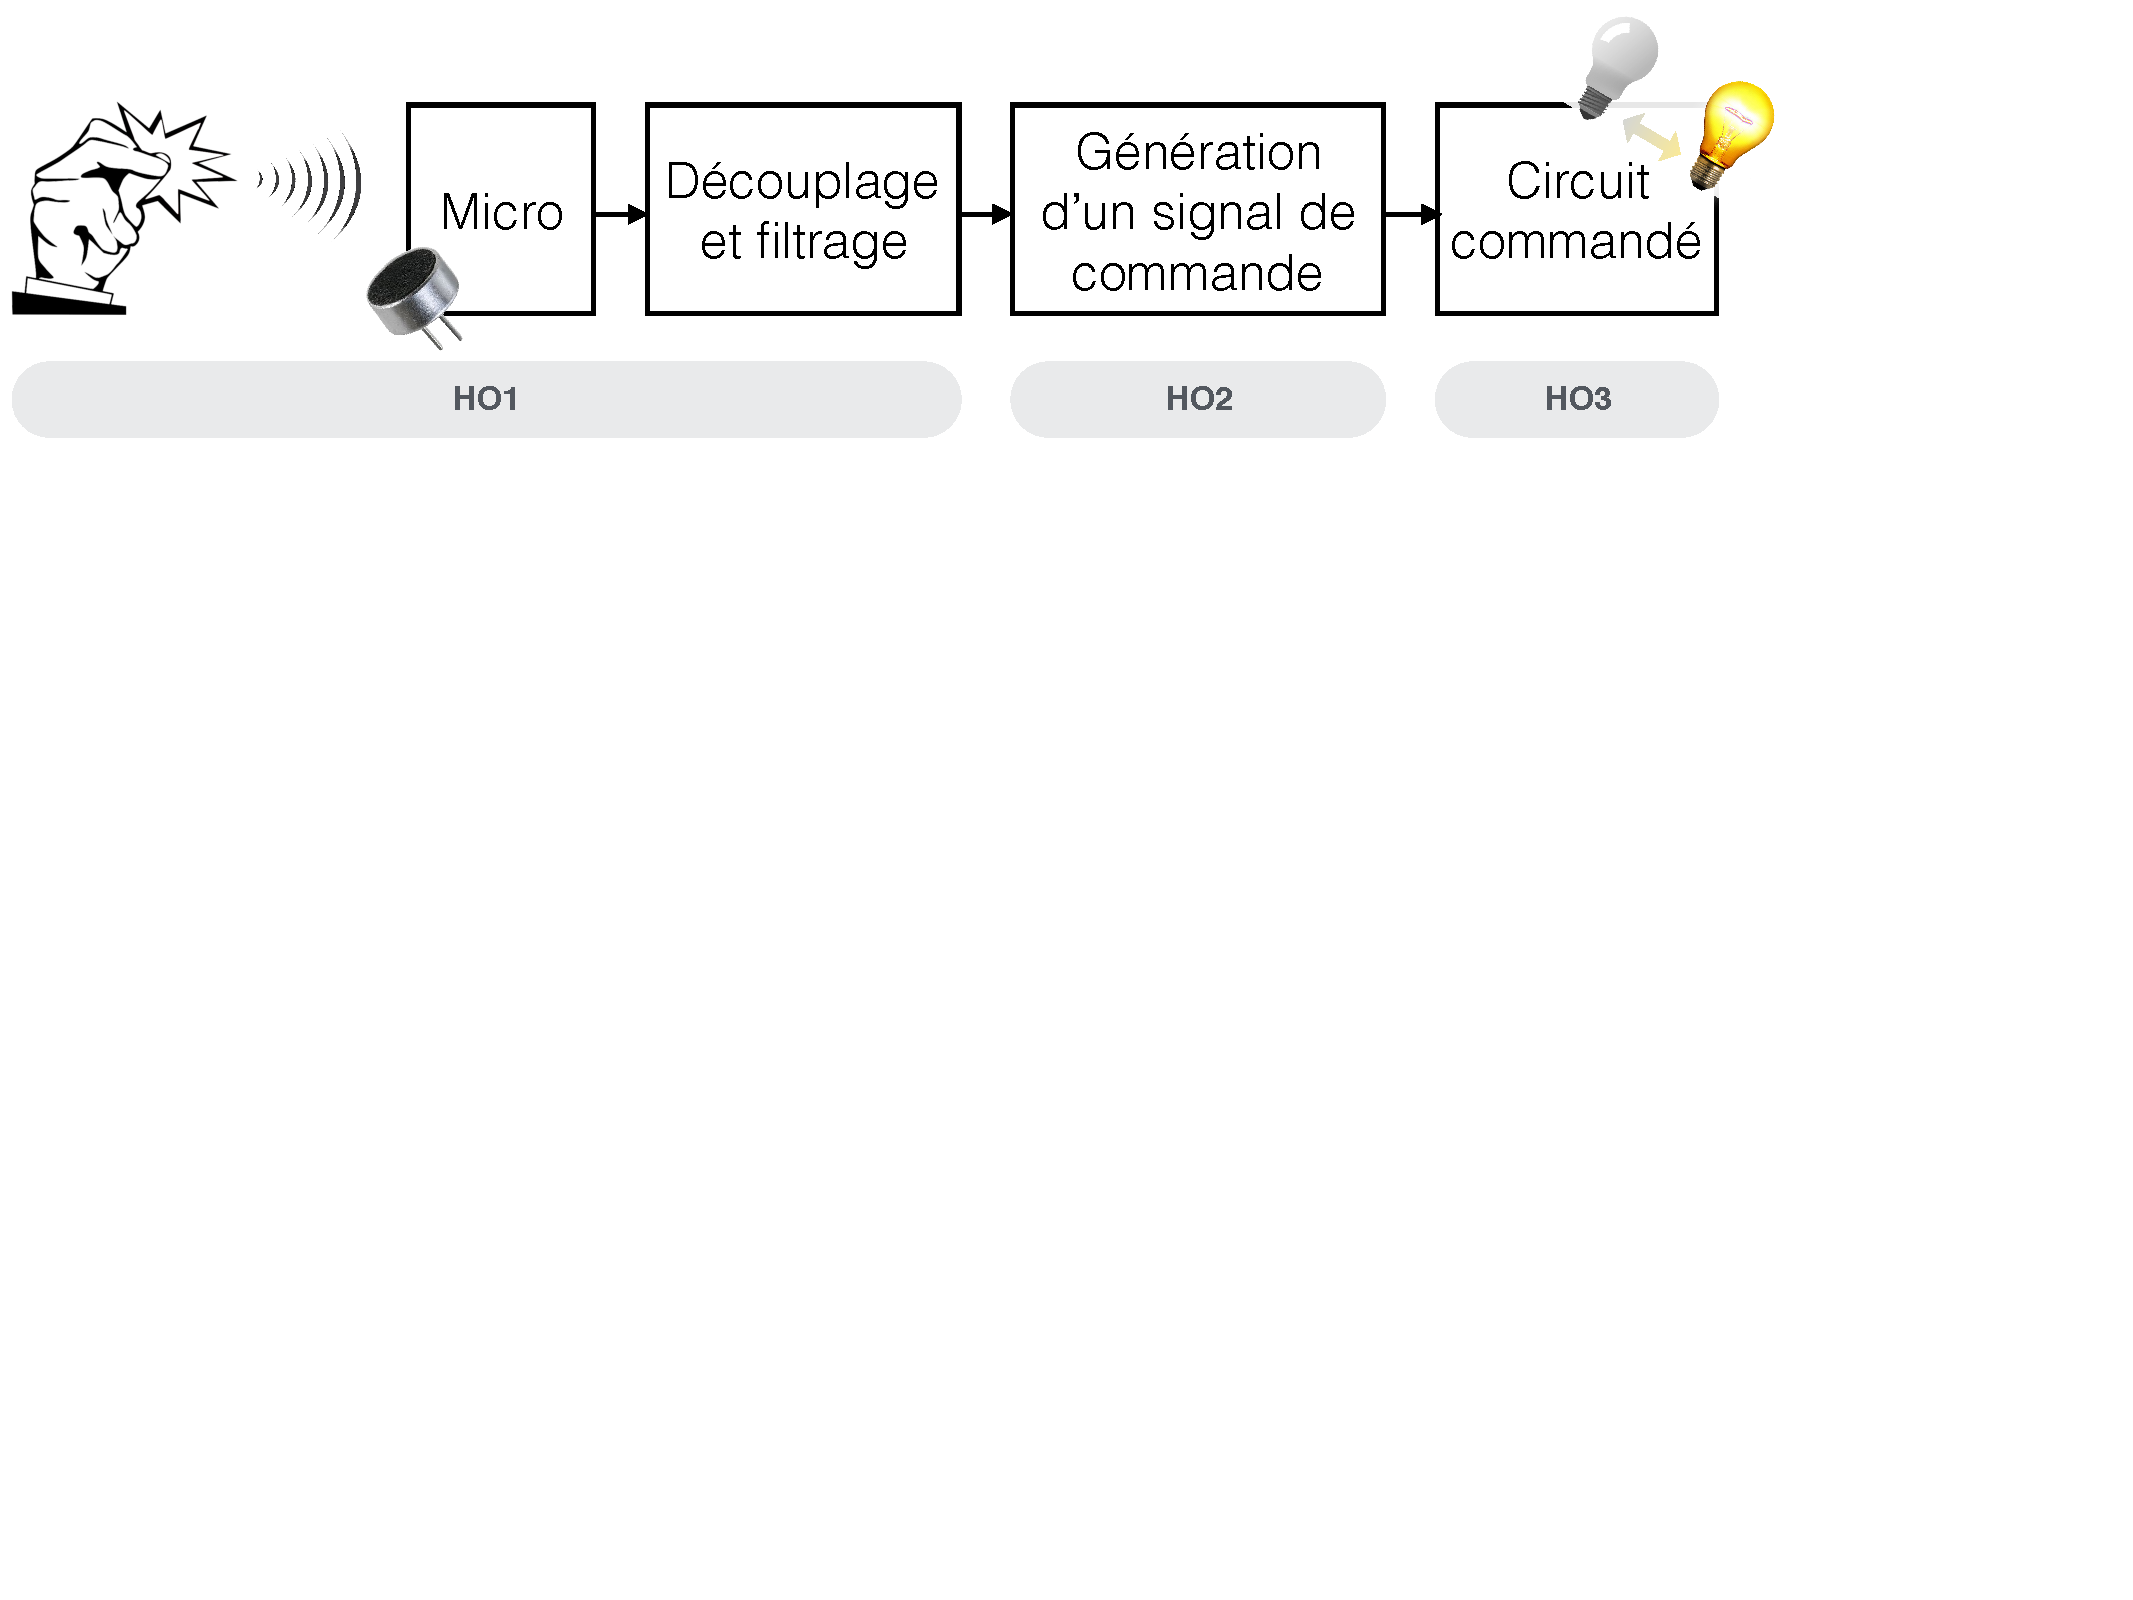
\includegraphics[width=.75\textwidth]{figures/SchemaBloc.pdf}
	\caption{Schéma-bloc du circuit.}
	\label{fig:block-diagram}
\end{figure}

Le schéma-bloc du circuit est présenté à la Figure \ref{fig:block-diagram}. Les ondes acoustiques générées par le claquement de doigt sont captées par le micro qui les transforme en un signal électrique (transduction). Ce signal est ensuite découplé et filtré à l'aide d'un filtre RC, comme présenté plus loin dans ce document. La génération d'un signal de commande propre ainsi que l'implémentation d'un circuit commandé seront abordées plus en détail dans les prochain hands-on.


%%% Microphone
\section{Microphone: du signal sonore au signal électrique}
% Principe de la transduction du signal sonore, du micro (electret microphone dans ce cas-ci), gamme de fréquence + schéma uniquement micro+résistance

Lorsque quelqu'un claque des doigts, une onde sonore est produite, qui consiste en fait en une variation locale de la pression de l'air qui se propage dans l'espace jusqu'à nos oreilles. Afin de commander un circuit électrique à partir de ce claquement de doigt, il est donc nécessaire de pouvoir transformer ce changement de pression en une variation d'une quantité électrique qu'il est possible de mesurer. Cette transformation d'une grandeur physique en une caractéristique électrique s'appelle la transduction. Dans le cas d'un signal sonore, cette transduction se fait à l'aide d'un dispositif bien connu: le microphone. \\

Il existe différents types de microphones (à ruban, à condensateur...) avec des fonctionnements, des performances et des prix différents. Celui mis à votre disposition pour ce projet est le modèle \texttt{ABM-707-RC}. Il s'agit d'un micro électrostatique à électret. C'est un micro qui s'adapte assez bien à un petit projet d'électronique au vu de sa petite taille, de son prix très démocratique et de sa grande facilité d'utilisation. \\

Un micro à électret se compose d'une membrane polarisée, c'est-à-dire qu'elle porte une charge électrostatique, d'une électrode et d'un circuit d'amplification. Lorsqu'une onde sonore arrive, elle va faire vibrer la membrane à l'intérieur du micro, ce qui va faire varier sa distance par rapport à l'électrode. Grâce au champ électrique généré par la membrane polarisée, un changement de tension va être produit sur l'électrode. Ce changement de tension sera ensuite amplifié par l'amplificateur avant de se retrouver à la sortie du micro.\\

Voici brièvement quelques caractéristiques techniques du micro utilisé:
\begin{itemize}
\item Ce micro nécessite une alimentation allant de 2 à 10V, utilisée pour son amplificateur interne. Dans ce projet, nous utiliserons une tension de 5V.
\item Ce micro couvre une plage de fréquences allant de 50 Hz à 16kHz, ce qui est largement suffisant pour l'application visée. Pour votre information, les humains perçoivent des fréquences allant (grossièrement) de 20 à 20 kHz.
\item Ce micro a une sensitivité de -41dB.
\item Ce micro est omnidirectionnel, c'est-à-dire qu'il entend aussi bien dans toutes les directions.
\end{itemize}



%%% Circuit
\section{Un circuit simple pour démarrer}
Le circuit que nous allons utiliser aujourd'hui se compose de quatre éléments:
\begin{enumerate}
  \item D'une télécommande infrarouges
  \item Récepteur infrarouges
  \item Une led
  \item L'Arduino qui est le \textit{"cerveau"} du système. Il allume la Led quand la télécommande lui demande.
\end{enumerate}

Pour que tout ceci fonctionne, la première étape est d'assembler tout ces composants sur une breadboard. Le schéma du circuit est disponible à la \ref{fig:circuit}.

\begin{figure}[!t]
\centering
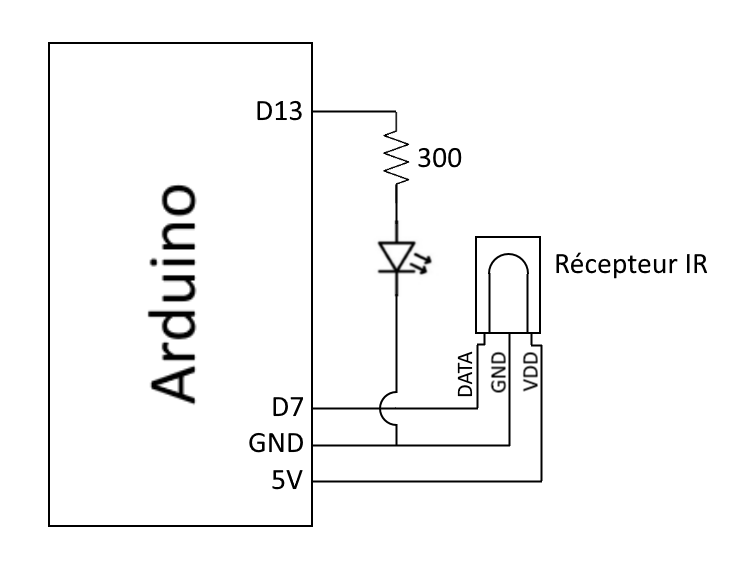
\includegraphics[width=0.8\textwidth]{imgs/circuit.png}
\caption{Circuit à réaliser pour contrôler l'Arduino grâce à une télécommande infrarouge.}
\label{fig:circuit}
\end{figure}


% Signal DC et AC
\section{Signal AC ou DC?}
% Signal AC ou DC? Explications, schéma

En électronique, on utilise souvent la notion de signal pour décrire l'information qui est transportée le long des fils du circuit. Ce signal représente en fait la valeur du courant ou de la tension dans un fil au cours du temps. Il existe énormément de façons de caractériser ce signal. Une distinction importante est la notion de signal DC ou AC. Un signal DC (de l'anglais \textit{Direct Current}) correspond à une valeur qui reste constante au cours du temps. Inversement, un signal AC (\textit{Alternating Current}) correspond à un signal qui va osciller au cours du temps d'une valeur positive à une valeur négative. Par exemple, comme illustré à la Figure \ref{fig:ACDC}, la tension au borne d'une pile est dite DC car la tension est constante à 1.5V. Dans une prise de courant par contre, on retrouve une tension AC qui oscille de -310V à +310V, 50 fois par seconde.\\

\begin{figure}[!ht]
	\centering
	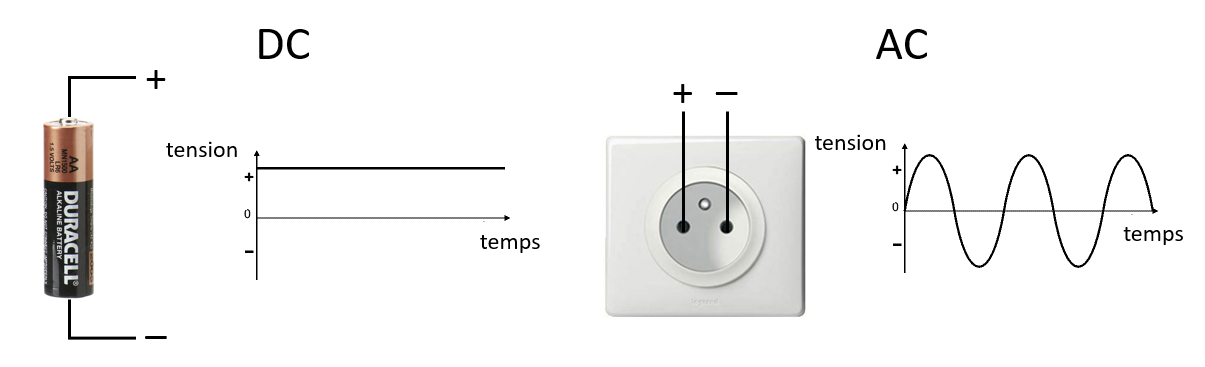
\includegraphics[width=\textwidth]{figures/AC-DC.PNG}
	\caption{Exemples de signaux DC et AC}
	\label{fig:ACDC}
\end{figure}

Dans le cas de notre micro, c'est encore un peu plus compliqué que cela. En effet, le signal produit par le micro reproduit les vibrations de l'air venant du son, et oscille donc bien comme un signal AC. Cependant, celui-ci est superposé à une tension DC (qui est due à l'électronique interne du micro, c'est un peu plus compliqué donc nous ne l'aborderons pas ici). Une illustration de ceci est présenté à la Figure \ref{fig:ACplusDC}, mais attention ce n'est pas à l'échelle!

\begin{figure}[!ht]
	\centering
	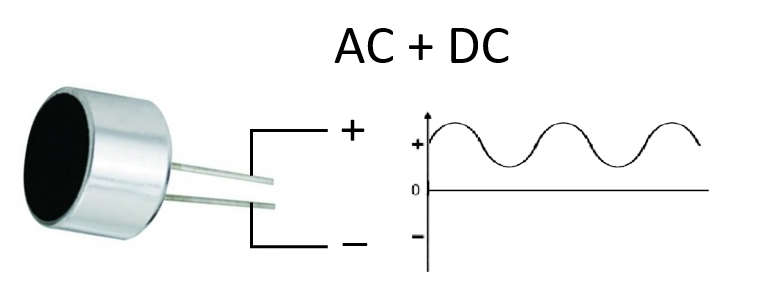
\includegraphics[width=.5\textwidth]{figures/microSignal.PNG}
	\caption{Signal AC superposé sur une tension DC}
	\label{fig:ACplusDC}
\end{figure}

% Oscilloscope
\section{A vous d'essayer!}
% Fonctionnement général de l'oscilloscope, prise en main, quelques manipulations pour observer le signal sur le microphone (en fonction du couplage, de l'amplitude, de l'échelle de temps...)

Assez d'explications théoriques, il est temps pour vous de passer à la pratique et d'essayer de mesurer les signaux produits par le microphone. Pour observer des signaux électriques, un instrument bien utile est l'oscilloscope. En connectant sa sonde (\textit{probe} en anglais) à un endroit du circuit, celui-ci affiche la tension en ce point au cours du temps. Il existe énormément de types d'oscilloscopes différents, des plus petits au plus complexes. Un oscilloscope est composé en général d'un écran sur lequel s'affiche le signal et de boutons de contrôle qui permettent de régler l'amplitude du signal affiché (en ordonnée sur le graphe) et l'échelle de temps (en abscisse). 

\begin{figure}[!ht]
	\centering
	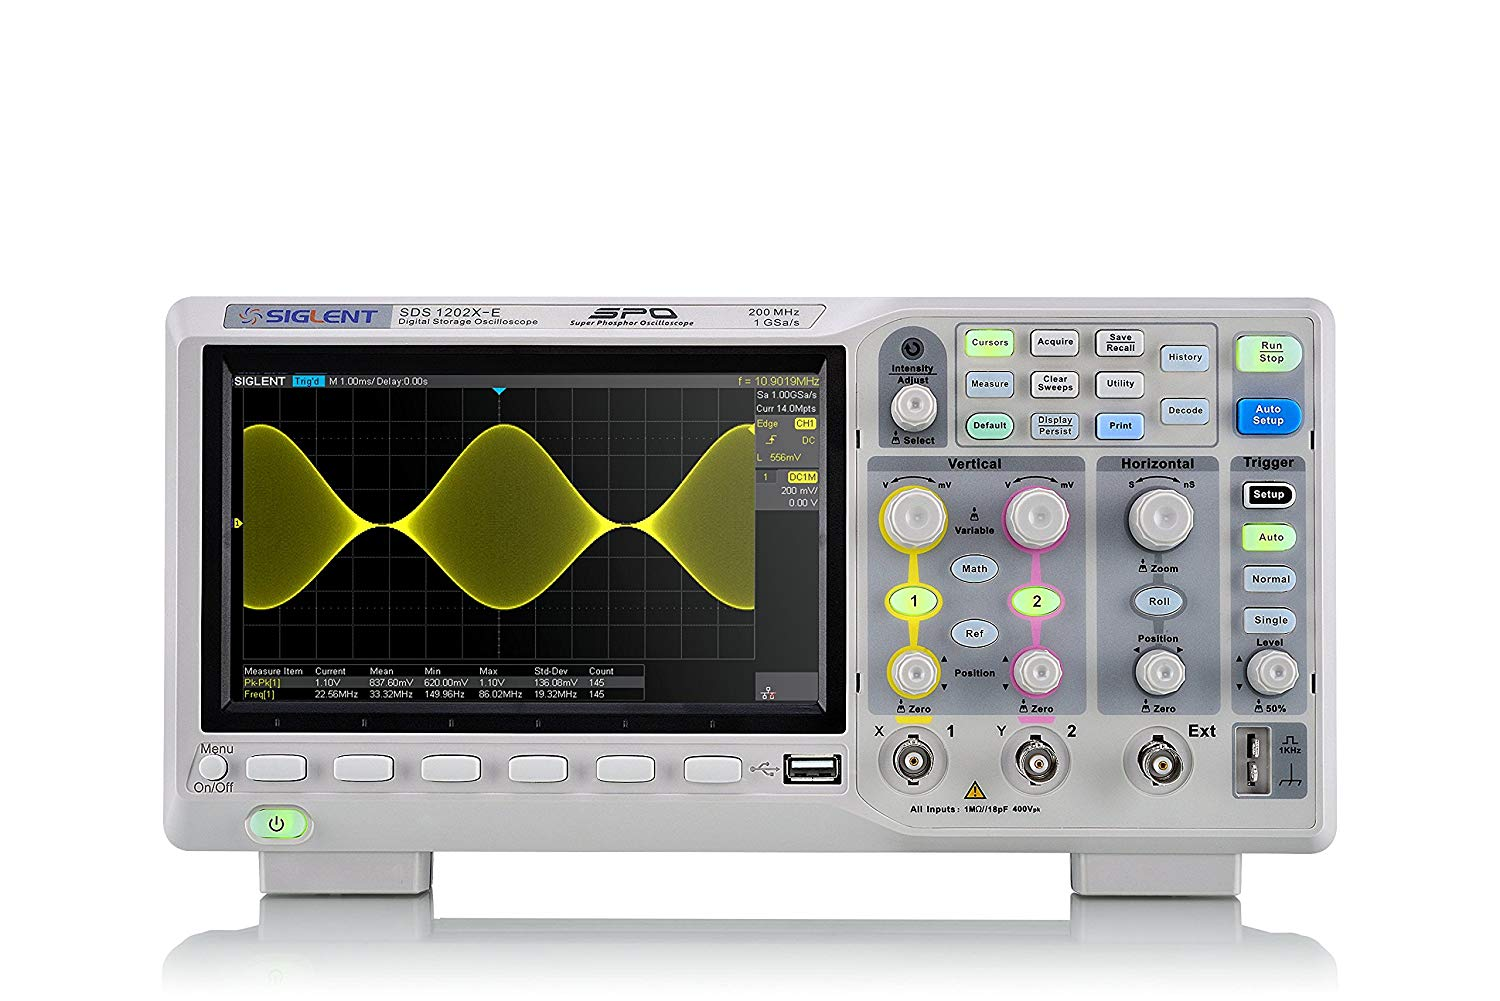
\includegraphics[width=.6\textwidth]{figures/oscillo.jpg}
	\caption{Oscilloscope}
	\label{fig:oscillo}
\end{figure}

L'affichage du signal fonctionne généralement en 2 modes différents: soit en mode continu où le signal défile sans arrêt sur l'écran, soit en mode déclenchable (\textit{trigger}) où le signal ne s'affiche que lorsqu'il dépasse un certain seuil. Ce deuxième mode est bien pratique pour observer des événements très brefs, tel que le signal sonore d'un claquement de doigts par exemple. \\

L'oscilloscope permet d'utiliser deux modes de couplage différents, appelés DC et AC (ça devrait te rappeler quelque chose...). Dans le mode DC, l'intégralité du signal est affiché à l'écran. \\

Les boutons correspondant à tous ces réglages sur chaque oscilloscopes sont différents d'une version à l'autre, appelle donc un membre du staff pour t'aider à t'y retrouver!\\

Pour chacun des signaux ci-dessous, réfléchis au réglage le plus approprié (amplitude, échelle de temps, mode continu ou déclenchable, découplage DC ou AC), et règle ensuite l'oscilloscope pour observer et mesurer le signal:
\begin{itemize}
\item La masse (référence de tension correspondant à 0V).
\item La tension d'alimentation à 5V.
\item La composante DC du signal de sortie du microphone.
\item La composante AC du signal de sortie du microphone.
\end{itemize}

% Filtrage
\section{Capacité, filtres et découplage}
% Schéma avec le filtre RC pour le découplage, fonctionnement, résultat, mesure à l'oscillo
Afin de supprimer la composante DC, il va nous falloir implémenter un filtre. Un filtre permet de choisir quelles fréquences du signal vont pouvoir passer. Ils permettent soit de ne laisser passer que les hautes, que les basses fréquences ou une bande de fréquences.
Dans ce cas-ci, nous voulons supprimer la constante qui correspond à une fréquence de zéro. Il va donc falloir implémenter un filtre passe haut. Ce filtre est réalisé grâce la capacité C1 et la résistance R2. La capacité est un composant qui accumule des charges électriques. C'est pourquoi, il ne peut y avoir que des variations de tensions à ces bornes. Donc la composante DC, qui ne varie pas, ne passe pas à travers la capacité. Le signal AC lui, n'est pas affecté par celle-ci. \\

Le signal filtré est récupéré aux bornes de la résistance. Vous pouvez observer l'effet du filtre grâce à oscilloscope. Placez une sonde avant le filtre et après le filtre pour voir son effet. 

\begin{figure}[!ht]
	\centering
	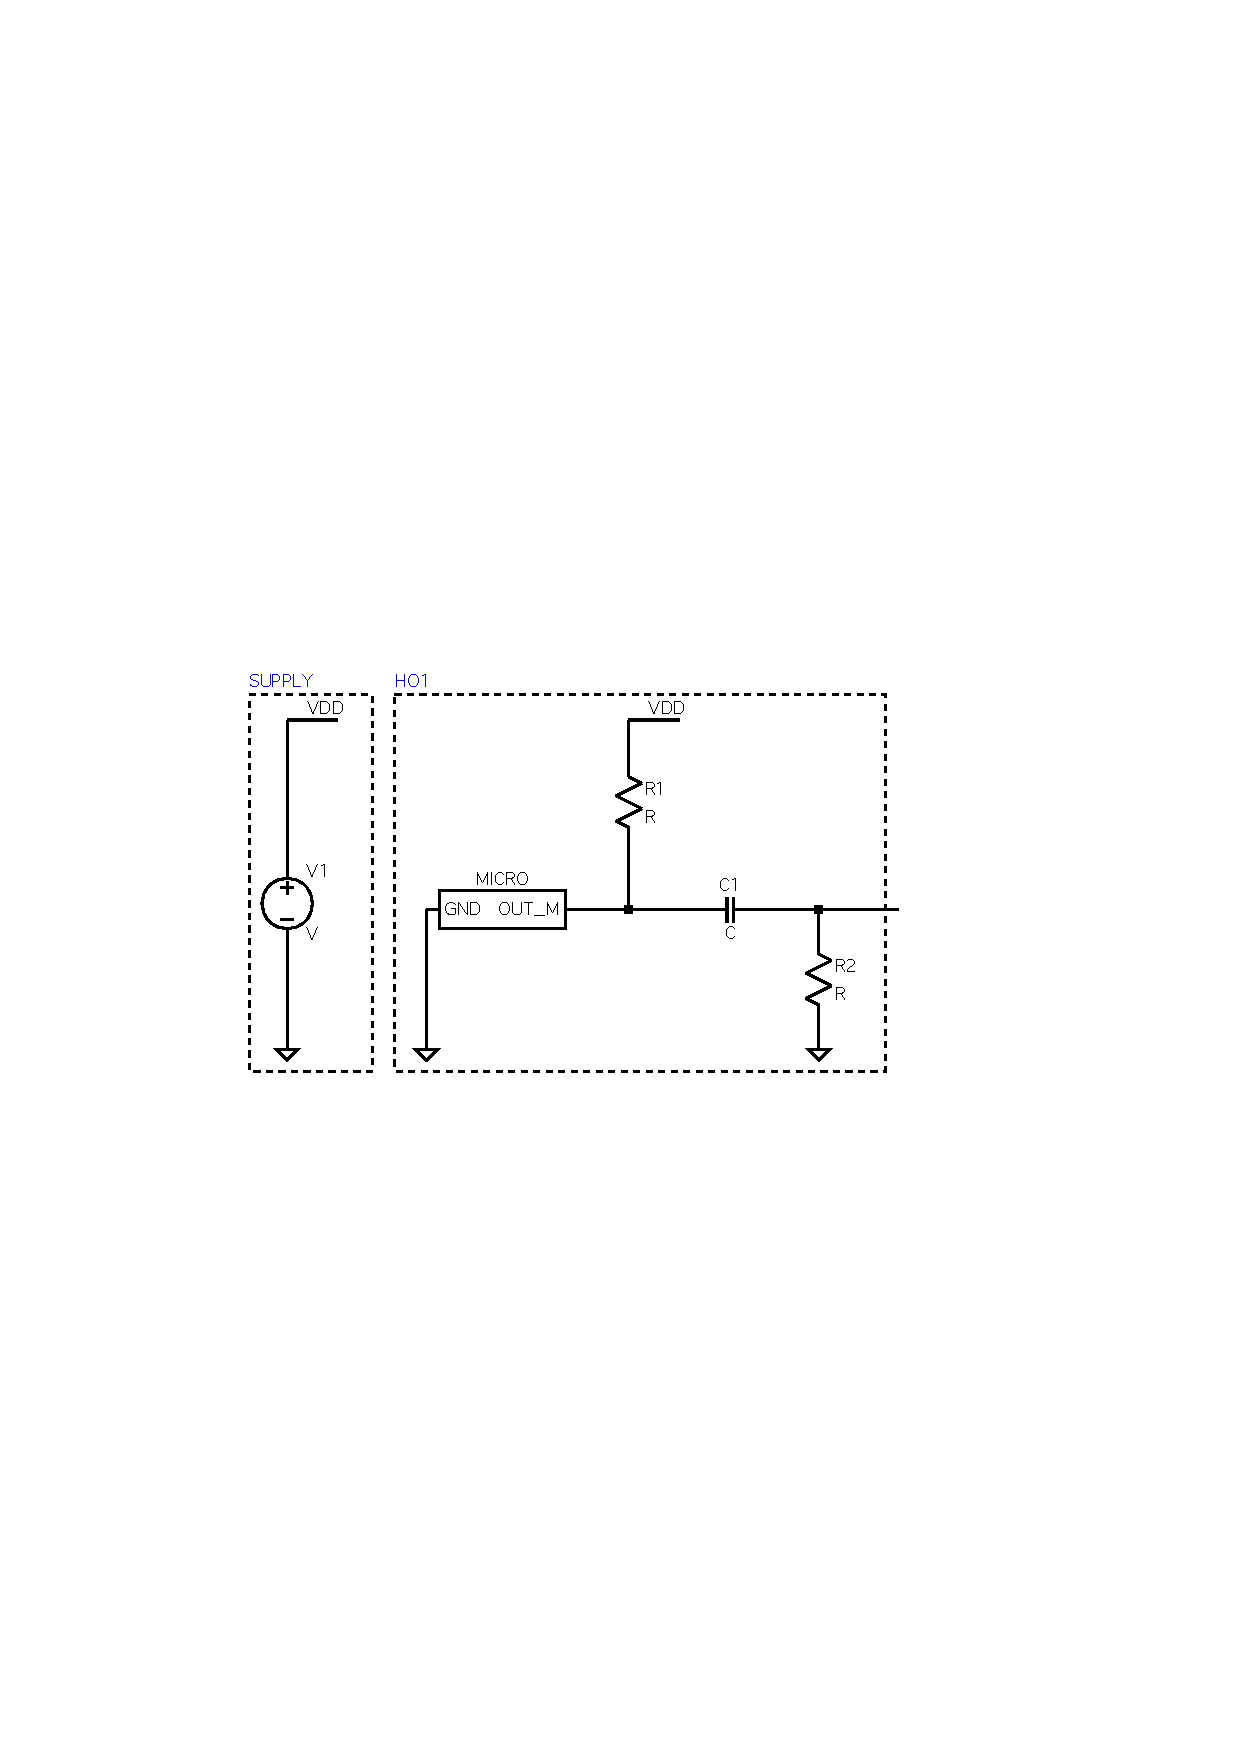
\includegraphics[width=.75\textwidth]{figures/Circuit_P1.pdf}
	\caption{Circuit HO1 avec filtre de découplage. $R2 = 55 k\Omega$, $C1 = 150n F$.}
	\label{fig:circuit_H01_filtre}
\end{figure}


% Réflexions sur le système
\section{Et après...}
% Réflexions sur quels blocs utiliser pour détecter ce signal

Vous savez maintenant comment transformer l'onde sonore du claquement de doigts en un signal électrique que vous pouvez filtrer et observer au microscope. Lors des prochains hands-on (la semaine prochaine), vous implémenterez le circuit qui permet de détecter automatiquement ce claquement. Selon vous, comment feriez-vous pour détecter ce signal, de manière générale sans penser encore à l'implémentation à l'aide de composants électroniques? Quelles "fonctions" électroniques utiliseriez-vous pour passer du signal observer aujourd'hui à un signal de commande tel qu'illustré ci-dessous?

\begin{figure}[!ht]
	\centering
	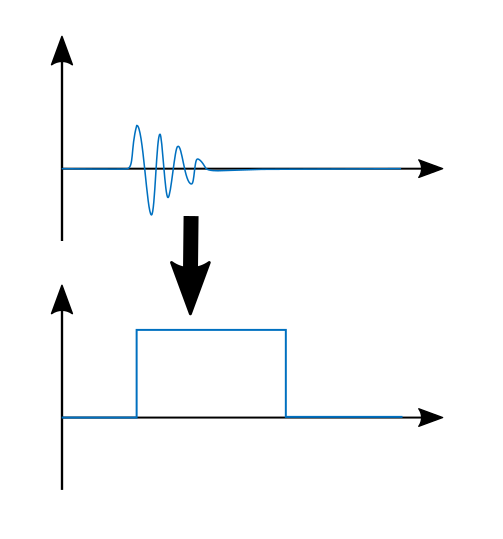
\includegraphics[width=.6\textwidth]{figures/signals.PNG}
	\caption{Détection d'un claquement de doigts}
	\label{fig:signals}
\end{figure}

\end{document}